\documentclass[border={0.1cm 0.1cm 0.1cm 0.1cm}]{standalone}  %E,S,W,N

\usepackage{amssymb}
\usepackage{amsmath}
\usepackage{tikz}
\usetikzlibrary{decorations.pathreplacing}	%for brackets

\begin{document}
	
	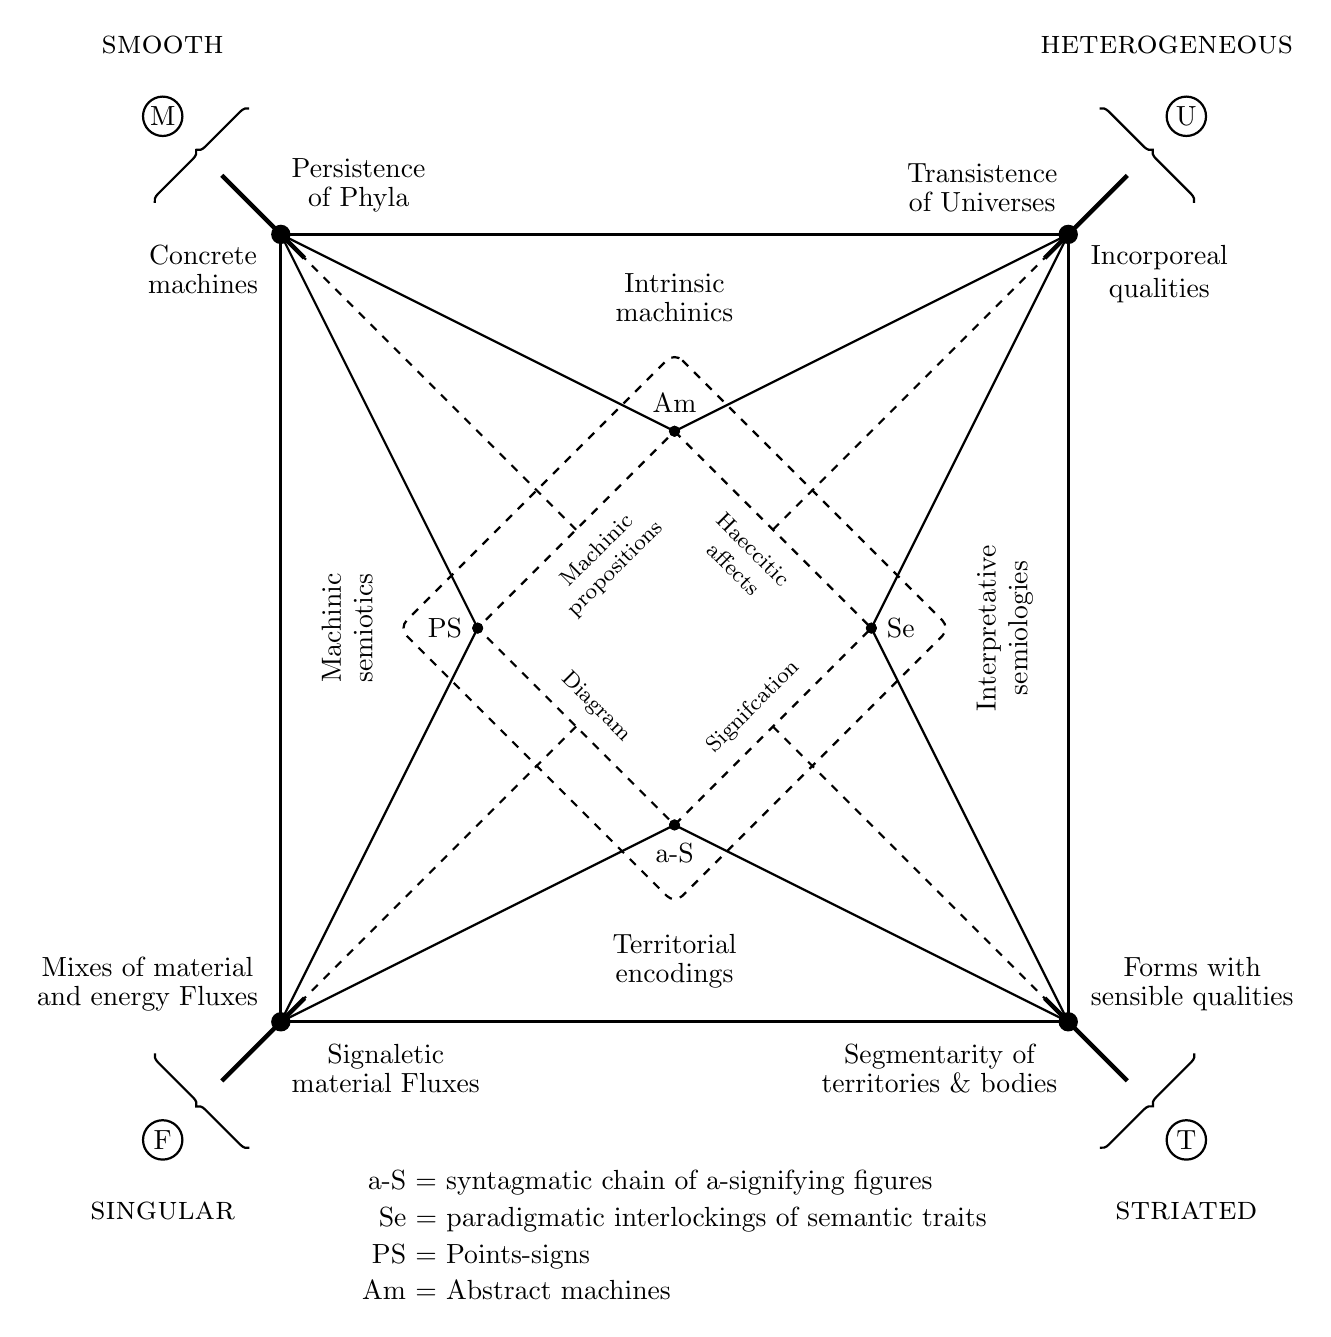
\begin{tikzpicture}[very thick]
	\def\s{5} %side of main square
	
	%MAIN SQUARE
	\draw (-\s,\s)--(\s,\s)--(\s,-\s)--(-\s,-\s)--cycle;
	\draw[thick] (-\s,\s)--(0,0.5*\s)--(\s,\s)--(0.5*\s,0)--(\s,-\s) --(0,-0.5*\s)--(-\s,-\s)--(-0.5*\s,0)--cycle;
	
	\foreach \i/\j/\l in {1/1/U,1/-1/T,-1/1/M,-1/-1/F}{
		\fill (\i*\s,\j*\s) circle (3.5pt);	
		\fill (0,0.5*\i*\s) circle (2pt);
		\fill (0.5*\i*\s,0) circle (2pt);
		\draw[dashed,thick] (0.25*\i*\s,0.25*\j*\s)--(\i*\s,\j*\s);
		\draw[ultra thick] (\i*\s-\i*0.3,\j*\s-\j*0.3)--(\i*\s+\i*0.75,\j*\s+\j*0.75);
		\draw[thick] (\i*1.3*\s,\j*1.3*\s) circle (0.25cm) node {\l};
	}
	
	%BRACKETS
	\draw[decorate,decoration={brace,amplitude=3pt},thick] (\s+1-0.6,\s+1+0.6)--(\s+1+0.6,\s+1-0.6);
	\draw[decorate,decoration={brace,amplitude=3pt},thick,xscale=-1] (\s+1+0.6,\s+1-0.6)--(\s+1-0.6,\s+1+0.6);
	\draw[decorate,decoration={brace,amplitude=3pt},thick] (\s+1+0.6,-\s-1+0.6)--(\s+1-0.6,-\s-1-0.6);
	\draw[decorate,decoration={brace,amplitude=3pt},thick,xscale=-1] (\s+1-0.6,-\s-1-0.6)--(\s+1+0.6,-\s-1+0.6);
	
	%INNER LABELS
	\draw[thick,dashed] (0,0.5*\s)--(0.5*\s,0)--(0,-0.5*\s)--(-0.5*\s,0)--cycle;
	\node[above,yshift= 1mm] at (0,0.5*\s)  {Am};
	\node[right,xshift=.6mm] at (0.5*\s,0)  {Se};
	\node[below,yshift=-1mm] at (0,-0.5*\s) {a-S};
	\node[left,xshift=-.6mm] at (-0.5*\s,0) {PS};
	%
	\draw[thick,dashed,rounded corners] (0,0.7*\s)--(0.7*\s,0)--(0,-0.7*\s)--(-0.7*\s,0)--cycle;
	\node[above,align=center] at (0,0.75*\s) {Intrinsic \\[-0.5mm] machinics};
	\node[right,align=center] at (0.74*\s,0) {\rotatebox{90}{Interpretative}};
	\node[right,align=center] at (0.82*\s,0) {\rotatebox{90}{semiologies}};
	\node[below,align=center] at (0,-0.75*\s) {Territorial \\[-0.5mm] encodings};
	\node[left,align=center] at (-0.82*\s,0) {\rotatebox{90}{Machinic}};
	\node[left,align=center] at (-0.74*\s,0) {\rotatebox{90}{semiotics}};
	%
	%\node at (-0.2*\s,0.2*\s) {\rotatebox{45}{\footnotesize Machinic propositions}};
	\node at (-0.2*\s,0.2*\s) {\rotatebox{45}{\footnotesize Machinic}};
	\node at (-0.15*\s,0.15*\s) {\rotatebox{45}{\footnotesize propositions}};
	%\node at (0.2*\s,0.2*\s) {\rotatebox{-45}{\footnotesize Haeccitic affects}};
	\node at (0.2*\s,0.2*\s) {\rotatebox{-45}{\footnotesize Haeccitic}};
	\node at (0.15*\s,0.15*\s) {\rotatebox{-45}{\footnotesize affects}};
	\node at (-0.2*\s,-0.2*\s) {\rotatebox{-45}{\footnotesize Diagram}};
	\node at (0.2*\s,-0.2*\s) {\rotatebox{45}{\footnotesize Signifcation}};
	
	%OUTER LABELS
	\node[align=center,above left,yshift=1.5mm] at (\s,\s) {Transistence \\[-0.5mm] of Universes};
	\node[align=center,below right,xshift=1.5mm] at (\s,\s) {Incorporeal \\ qualities};
	%
	\node[align=center,above right,yshift=1.5mm] at (-\s,\s) {Persistence \\[-0.5mm] of Phyla};
	\node[align=center,below left,xshift=-1.5mm] at (-\s,\s) {Concrete \\[-0.5mm] machines};
	%
	\node[align=center,above left,xshift=-1.5mm] at (-\s,-\s) {%
		Mixes of material \\[-0.5mm] and energy Fluxes
	};
	\node[align=center,below right,yshift=-1.5mm] at (-\s,-\s) {%
		Signaletic \\[-0.5mm] material Fluxes
	};
	%
	\node[align=center,above right,xshift=1.5mm] at (\s,-\s) {%
		Forms with \\[-0.5mm] sensible qualities
	};
	\node[align=center,below left,yshift=-1.5mm] at (\s,-\s) {%
		Segmentarity of \\[-0.5mm] territories \& bodies
	};
	%
	\node at (-1.3*\s, 1.48*\s) {\large\scshape smooth};
	\node at ( 1.3*\s,-1.48*\s) {\large\scshape striated};
	\node at (1.25*\s, 1.48*\s) {\large\scshape heterogeneous};
	\node at (-1.3*\s,-1.48*\s) {\large\scshape singular};
	
	%LEGEND
	\node[align=left,below] at (0,-1.35*\s) {%
		\hspace{2pt}a-S = syntagmatic chain of a-signifying figures\\[0.5mm]
		\hspace{6pt}Se = paradigmatic interlockings of semantic traits\\[0.5mm]
		\hspace{3.5pt}PS = Points-signs\\[0.25mm]
		Am = Abstract machines
	};
	\end{tikzpicture}
	
\end{document}